\documentclass[]{article}

\usepackage[italian]{babel}
\usepackage[margin=20mm, footskip = 20pt]{geometry}
\usepackage{array}
\usepackage{tabularx}
\usepackage{graphicx}
\usepackage{subfiles}
\usepackage{hyperref}
\usepackage{nameref}
\usepackage{titlesec}
\usepackage{longtable}
\usepackage[table]{xcolor}
\usepackage{titling}
\usepackage{lastpage}
\usepackage{ifthen}
\usepackage{calc}
\usepackage{soulutf8}
\usepackage{contour}
\usepackage{float}
\usepackage{fancyhdr}
\usepackage{multirow}
\usepackage{pgfgantt}
\usepackage{lscape}

\newcommand{\hr}{\par\vspace{-.1\ht\strutbox}\noindent\hrulefill\par}

\graphicspath{ {./}
	{./commons/res}
}

%--------------------------------------------------
% Comandi per inserire contenuto del documento
%--------------------------------------------------
\makeatletter

\newcommand\appendToGraphicsPath[1]{%
	\g@addto@macro\Ginput@path{{#1}}%
}

\newcommand{\setTitle}[1]{%
	\newcommand{\@phTitle}{#1}%
}
\newcommand{\phTitle}{\@phTitle}

\newcommand{\setDate}[1]{%
	\newcommand{\@phDate}{#1}%
}
\newcommand{\phDate}{\@phDate}

\newcommand{\setUso}[1]{%
	\newcommand{\@uso}{#1}%
}
\newcommand{\uso}{\@uso}

\newcommand{\setVersione}[1]{%
	\newcommand{\@versione}{#1}%
}
\newcommand{\versione}{\@versione}

\newcommand{\disabilitaVersione}{%
	\renewcommand{\setVersione}[1]{}%
	\renewcommand{\versione}{DISABILITATA}
}

\newcommand{\setResponsabile}[1]{%
	\newcommand{\@responsabile}{#1}%
}
\newcommand{\responsabile}{\@responsabile}

\newcommand{\setRedattori}[1]{%
	\newcommand{\@redattori}{#1}%
}
\newcommand{\redattori}{\@redattori}

\newcommand{\setVerificatori}[1]{%
	\newcommand{\@verificatori}{#1}%
}
\newcommand{\verificatori}{\@verificatori}

\newcommand{\setModifiche}[1]{%
	\newcommand{\@modifiche}{#1}%
}
\newcommand{\modifiche}{\@modifiche}

\makeatother 

%--------------------------------------------------
% Comandi per i documenti esterni e il glossario
%--------------------------------------------------

\newcommand{\dext}[1]{\textsc{#1\textsubscript{\textit{D}}}}

\newcommand{\glock}[1]{\textsc{#1\textsubscript{\textit{G}}}}

%--------------------------------------------------
% Comandi per impostare sottotitoli di quarto e quinto livello
%--------------------------------------------------

\setcounter{secnumdepth}{4}
\setcounter{tocdepth}{4}

\titleformat{\paragraph}
{\normalfont\normalsize\bfseries}{\theparagraph}{1em}{}
\titlespacing*{\paragraph}{0pt}{2.25ex plus 1ex minus .2ex}{1.5ex plus .2ex}

\titleformat{\subparagraph}
{\normalfont\normalsize\bfseries}{\thesubparagraph}{1em}{}
\titlespacing*{\subparagraph}{0pt}{1.75ex plus 1ex minus .2ex}{.75ex plus .1ex}

\appendToGraphicsPath{../../commons/res/}

%------------------------------
%
% COMANDI DI CONFIGURAZIONE
%
%------------------------------

\setTitle{Norme di Progetto}

\setVersione{0.6.0}

\setDate{26-12-2020}

\setResponsabile{Paolo Scanferlato}

\setRedattori{Matteo Alba \\&
	Giacomo Bulbarelli \\&
	Alessandro Chimetto \\&
	Alessandro Dindinelli \\&
	Lucia Fenu \\&
	Paolo Scanferlato \\&
	Valton Tahiraj}

\setVerificatori{Alessandro Chimetto \\&
  Valton Tahiraj}

\setUso{Interno}

\setModifiche{
	0.3.0 & Alessandro Chimetto		& Amministratore& 20-12-2020 & Aggiunto processo di Gestione della Configurazione\\
    0.6.0 & Alessandro Chimetto     & Verificatore  & 26-12-2020 & Verificati processi di Verifica e Validazione\\
	0.6.0 & Giacomo Bulbarelli      & Amministratore& 26-12-2020 & Aggiunto sezione Verifica e sezione Validazione\\
	0.5.0 & Valton Tahiraj 			& Verificatore  & 26-12-2020 & Verificato Gestione Processi\\
	0.5.0 & Lucia Fenu 				& Amministratore& 26-12-2020 & Aggiunto Gestione Processi\\
    0.4.0 & Alessandro Chimetto     & Verificatore  & 24-12-2020 & Verificato Processo di Formazione Personale\\
	0.4.0 & Valton Tahiraj 			& Amministratore& 24-12-2020 & Aggiunto Formazione Personale \\
	0.3.0 & Alessandro Chimetto     & Verificatore  & 24-12-2020 & Verificato Processo di Sviluppo\\
	0.3.0 & Alessandro Dindinelli	& Amministratore& 23-12-2020 & Aggiunto Processo di Sviluppo\\
	0.2.0 & Alessandro Chimetto		& Verificatore	& 21-12-2020 & Verificato Processo di Fornitura\\
	0.2.0 & Valton Tahiraj 			& Amministratore& 20-12-2020 & Aggiunto Processo di Fornitura \\
	0.1.0 & Alessandro Chimetto		& Verificatore	& 15-12-2020 & Verificata Introduzione\\
	0.1.0 & Valton Tahiraj 			& Amministratore& 14-12-2020 & Aggiunto Introduzione \\
	0.0.0 & Alessandro Chimetto		& Verificatore	& 14-12-2020 & Verifica prima stesura\\
	0.0.0 & Valton Tahiraj 			& Amministratore& 14-12-2020 & Prima stesura
}

\begin{document}
	% Direttive per la creazione del titolo tramite comando maketitle
\title{\huge \textsc{\phTitle{}} \\
	\vspace{11pt} \large \textsc{\phDate{}}}

\author{} % Non toccare
\date{} % Non toccare

%--------------------
% Frontespizio
%--------------------

% Logo del gruppo
\begin{figure}[t!]
	\centering
	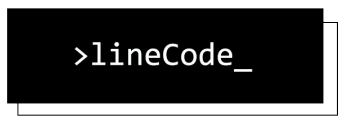
\includegraphics[width=20em]{lclong}
\end{figure}

% Titolo / Nome
\maketitle
\thispagestyle{empty}

% Dati specifici sul doc in forma tabulare
\begin{table}[ht]
	\begin{center}
		\label{tab:Dati sul documento}
		\begin{tabular}{r|l}
			\multicolumn{2}{c}{ \textsc{Dati sul documento} } \\
			\hline
			\textbf{Versione} & \versione{} \\
			\textbf{Uso} & \uso{}  \\
			\textbf{Redattori} & \redattori{} \\
			\textbf{Verificatori} & \verificatori{} \\
			\textbf{Responsabile} & \responsabile{} \\
			\textbf{Destinatari} & lineCode \\
								& prof.\ Vardanega Tullio \\		
								& prof.\ Cardin Riccardo \\
			\ifthenelse{\equal{\uso}{Esterno}}{
								& Sanmarco Informatica
			}{} \\
		\end{tabular}
	\end{center}
\end{table}

\newpage

\renewcommand{\arraystretch}{2} % allarga le righe con dello spazio sotto e sopra
\begin{longtable}[H]{>{\centering\bfseries}m{2cm} >{\centering}m{3.5cm} >{\centering}m{2.5cm} >{\centering}m{3cm} >{\centering\arraybackslash}m{5cm}}
	\rowcolor{lightgray}
	{\textbf{Versione}} & {\textbf{Nominativo}} & {\textbf{Ruolo}} & {\textbf{Data}} & {\textbf{Descrizione}}  \\
	\endfirsthead%
	\rowcolor{lightgray}
	{\textbf{Versione}} & {\textbf{Nominativo}}  & {\textbf{Ruolo}} & {\textbf{Data}} & {\textbf{Descrizione}}  \\
	\endhead%
	\modifiche{}%
\end{longtable}
	\newpage
	%--------------------------------
	%
	% IL CONTENUTO INIZIA DA QUI
	%
	%--------------------------------

	\section{Introduzione}
	\subsection{Scopo del documento}
Il documento ha lo scopo di definire le guidelines del way of working adottato dal team lineCode. Le attività presenti in questo documento sono redatte da processi contenuti nello standard ISO/IEC 12207:1995. Risulta quindi necessario che tutti i membri del gruppo prendano visione di questo documento ai fini di coesione e uniformità all'interno del progetto.

\subsection{Scopo del prodotto}
Il \glock{capitolato} C5 ha come obbiettivo la realizzazione di un applicativo \glock{Real-Time} in grado di guidare delle unità dotate di mobilità autonoma in ambienti specifici, partendo dal presupposto che queste si muovano in ambienti in cui sono presenti altre unità (autonome o meno).

\subsection{Glossario e documenti esterni}
In supporto alla documentazione viene fornito un glossario per chiarire, con una definizione, eventuali termini specifici contenuti in questo documento.
Saranno adottati quindi questi due simboli a pedice:
\begin{itemize}
	\item \textit{D} se indicano un documento specifico;
	\item \textit{G} se incluse nel \dext{glossario}.
\end{itemize}

\subsection{Riferimenti}
	\subsubsection{Riferimenti normativi}
	\begin{itemize}
		\item \textbf{{C5 - PORTACS}}: \url{https://www.math.unipd.it/~tullio/IS-1/2020/Progetto/C5.pdf};
        \item \textbf{Oracle Java Code Conventions}: \url{https://www.oracle.com/technetwork/java/codeconventions-150003.pdf};
        \item \textbf{Angular coding style guide}: \url{https://angular.io/guide/styleguide}.
	\end{itemize}
	\subsubsection{Riferimenti informativi}
	\begin{itemize}
		\item \textbf{ISO/IEC 12207:1995}: \url{https://www.math.unipd.it/~tullio/IS-1/2009/Approfondimenti/ISO_12207-1995.pdf};
		\item \textbf{Gitflow}: \url{http://nvie.com/posts/a-successful-git-branching-model/};
		\item \textbf{Documentazione Zapier}: \url{https://zapier.com/help};
		\item \textbf{Documentazione act}: \url{https://github.com/nektos/act/blob/master/README.md};
		\item \textbf{Studio di Fattibilità}: \dext{Studio di Fattibilità v1.0.0};
		\item \textbf{Piano di Qualifica}: \dext{Piano di Qualifica v2.0.0};
		\item \textbf{Piano di Progetto}: \dext{Piano di Progetto v2.0.0}.
	\end{itemize}
	\newpage

	\section{Processi primari}
	\subsection{Fornitura}

	\subsubsection{Obiettivi}
	L'obiettivo di questa sezione è descrivere le norme che il gruppo lineCode si impegna a rispettare per potersi proporre come fornitore nei confronti di Sanmarco Informatica SpA e dei committenti Prof. Tullio Vardanega e Prof. Riccardo Cardin per la progettazione, sviluppo e consegna del progetto \glock{portacs}

	\subsubsection{Attività}
		\paragraph{Studio di fattibilità}
		Documento che riporta lo studio svolto dagli analisti sui \glock{capitolati} proposti. Per ciascun \glock{capitolato} viene riportato:
		\begin{itemize}
			\item \textbf{Descrizione:} sintesi del prodotto richiesto da sviluppare presentato nel \glock{capitolato};
		 	\item \textbf{Finalità:} ambito di utilizzo del prodotto da sviluppare;
		 	\item \textbf{Tecnologie interessate:} lista di tutte le tecnologie interessate nello sviluppo del prodotto;
		 	\item \textbf{Analisi motivazione, criticità e rischi:} racchiude le motivazioni, le criticità e i rischi risultati dall'analisi del \glock{capitolato};
		 	\item \textbf{Valutazione finale:} indica le motivazioni per le quali il \glock{capitolato} è stato respinto o accettato.
		\end{itemize}

		\paragraph{Documentazione esterna}
		Il gruppo lineCode si impegna a fornire al proponente Sanmarco Informatica SpA e ai committenti Prof. Tullio Vardanega e Prof. Riccardo Cardin i seguenti documenti:
		\begin{itemize}
		 	\item \textbf{Piano di progetto:} documento che descrive le metodologie di pianificazione, consegna e completamento del progetto;
		 	\item \textbf{Piano di qualifica:} documento che contiene le attività di verifica, validazione e garantisce la qualità dei processi e di prodotto;
		 	\item \textbf{Analisi dei requisiti:} documento contenente l'analisi dei requisiti e dei casi d'uso del gruppo.
		\end{itemize}

	\subsubsection{Rapporto con il proponente}
	Il gruppo intende instaurare un dialogo costante ed un profondo rapporto di collaborazione con il proponente Sanmarco Informatica SpA, al fine di:
	\begin{itemize}
		\item determinare i bisogni del proponente;
		\item stabilire vincoli e  requisiti dei processi;
		\item stabilire vincoli e requisiti del prodotto;
		\item stimare tempistiche e costi del lavoro;
		\item accordarsi sulla qualifica di prodotto;
		\item chiarire eventuali dubbi emersi.
	\end{itemize}
	\newpage

	\subsection{Sviluppo}

	\subsubsection{Scopo}
	Questa sezione raccoglie le linee guida per i compiti e le attività da svolgere al fine di ottenere il prodotto finale richiesto dal proponente. \\
	Per implementare correttamente il processo si devono stabilire i seguenti punti:
	\begin{itemize}
		\item obiettivi di sviluppo;
		\item vincoli tecnologici e di design.
	\end{itemize}
	Il prodotto finale deve:
	\begin{itemize}
		\item rispettare i requisiti;
		\item superare i test definiti;
		\item soddisfare le richieste del proponente.
	\end{itemize}
	\subsubsection{Descrizione}
	Secondo lo standard ISO/IEC 12207:1995, il processo di sviluppo si divide in:
	\begin{itemize}
		\item Analisi dei Requisiti;
		\item Progettazione;
		\item Codifica.
	\end{itemize}

	\subsubsection{Attività}

		\paragraph{Analisi dei requisiti}
			\subparagraph{Scopo}
			Il compito degli analisti è quello di redigere il documento \dext{Analisi dei Requisiti v1.0.0}, che andrà ad elencare e definire i requisiti del \glock{capitolato}. Lo scopo dei requisiti è quello di:
			\begin{itemize}
				\item descrivere il prodotto da realizzare;
				\item rendere disponibili ai progettisti riferimenti precisi;
				\item esprimere casi d'uso e requisiti concordati;
				\item rendere disponibili ai verificatori riferimenti per il controllo dei test;
				\item ragionare sul lavoro richiesto per produrre una stima dei costi.
			\end{itemize}
			\subparagraph{Classificazione dei requisiti}
			Ogni requisito sarà associato ad un identificativo che rispetterà il seguente formato:
			\begin{center}
				\textbf{R[Priorità]-[Categoria]-[Codice]}
			\end{center}
			\begin{itemize}
				\item \textbf{R:} requisito;
				\item \textbf{Priorità:}
				\begin{itemize}
					\item \textbf{M:} mandatory/obbligatorio, quindi necessario a garantire le funzioni base del prodotto;
					\item \textbf{D:} desirable/desiderabile, cioè non strettamente necessario, ma che porta alla completezza del prodotto;
					\item \textbf{O:} optional/opzionale, quindi che non pregiudica la funzionalità del prodotto finale.
				\end{itemize}
				\item \textbf{Categoria:}
				\begin{itemize}
					\item \textbf{F:} functional/funzionale;
					\item \textbf{P:} performance/prestazionale;
					\item \textbf{Q:} qualitative/qualitativo;
					\item \textbf{C:} constraint/vincolo.
				\end{itemize}
				\item \textbf{Codice:} numero progressivo per riconoscere univocamente il requisito.
			\end{itemize}
			\subparagraph{Classificazione dei casi d'uso}
			Come per i requisiti, si prevede di identificare univocamente i casi d'uso con il seguente formato:
			\begin{center}
				\textbf{UC[Codice]}
			\end{center}
			\begin{itemize}
				\item \textbf{UC:} use case/caso d'uso;
				\item \textbf{Codice:} serie di cifre separate da ’.’ così da poter dividere in modo gerarchico i casi e sotto casi.
			\end{itemize}
			Oltre all'identificativo, ogni caso d'uso verrà approfondito dai seguenti campi:
			\begin{itemize}
				\item \textbf{Descrizione:} breve spiegazione della situazione modellata;
				\item \textbf{Grafici \glock{UML}:} diagrammi realizzati usando la versione 2.0 del linguaggio;
				\item \textbf{Attori:} gli attori primari e secondari coinvolti;
				\item \textbf{Scenario Principale:} elenco numerato degli eventi descritti dal caso d'uso;
				\item \textbf{Precondizione:} condizioni che si assumono vere prima che si verifichino gli eventi descritti dal caso d'uso;
				\item \textbf{Postcondizione:} condizioni che si assumono vere dopo che si sono verificati gli eventi descritti dal caso d'uso;
				\item eventuali estensioni ed inclusioni coinvolte.
			\end{itemize}

			\paragraph{Progettazione}
			\subparagraph{Scopo}
			Mentre l'\dext{Analisi dei Requisiti v1.0.0} divide il problema in parti per capirne completamente il dominio applicativo, la Progettazione rimette insieme tali parti specificandone le funzionalità in modo da realizzare l'architettura che il prodotto finale dovrà seguire. Questa dovrà seguire i seguenti principi:
			\begin{itemize}
				\item rispetto di tutti i requisiti;
				\item affidabilità nello svolgere i propri compiti;
				\item possibilità e facilità di garantire la manutenzione nel tempo;
				\item essere sicura rispetto ad intrusioni e malfunzionamenti;
				\item avere componenti coese, incapsulate e con scarse dipendenze tra loro.
			\end{itemize}
			\subparagraph{Descrizione}
			Possiamo dividere questa fase in due istanze principali:
			\begin{itemize}
				\item \textbf{Technology baseline}: contiene le specifiche della progettazione ad alto livello del prodotto, i diagrammi \glock{UML} utilizzati per la realizzazione dell'architettura ed i test di verifica;
				\item \textbf{Product baseline}: approfondisce ulteriormente l'attività di progettazione integrando la technology baseline e definisce i test necessari alla verifica.
			\end{itemize}
			\subparagraph{Technology baseline}
			Le componenti principali che individuiamo sono:
			\begin{itemize}
				\item diagrammi \glock{UML}, utilizzati per rendere più chiare le soluzioni progettuali utilizzate, possono essere diagrammi di classi, package, attività o sequenza;
				\item descrizione delle tecnologie adottate, specificandone l'utilizzo nel progetto, i vantaggi e gli svantaggi;
				\item \glock{design patterns} per adottare opportune soluzioni progettuali a problemi ricorrenti;
				\item test di integrazione, per verificare che ogni componente del sistema funzioni nella maniera voluta.
			\end{itemize}
			\subparagraph{Product baseline}
			Gli aspetti principali su cui soffermarsi sono:
			\begin{itemize}
				\item definizione delle classi e loro descrizione per scopo e funzionalità;
				\item tracciamento delle classi, in modo che per ogni requisito esista una classe che lo soddisfa;
				\item test di unità, definiti in modo da verificare che le parti funzionino individualmente nel modo stabilito.
			\end{itemize}

			\paragraph{Codifica}
			\subparagraph{Scopo}
			Questa parte ha lo scopo di realizzare il prodotto software richiesto. I programmatori dovranno attenersi a queste norme durante la fase di programmazione ed implementazione.
			\subparagraph{Descrizione}
			La scrittura del codice dovrà rispettare delle linee guida in modo da ottenere codice leggibile ed uniforme per i programmatori, ed agevolare poi le fasi di manutenzione, verifica e validazione. \\
			Le convenzioni principali comprendono:
			\begin{itemize}
				\item regole per la dichiarazione e la denominazione di variabili e funzioni;
				\item definizione degli standard di indentazione, spazi e commenti;
				\item prassi e principi di programmazione.
			\end{itemize}
	\newpage

	\section{Processi di Supporto}
	\subsection{Documentazione}

	\subsubsection{Descrizione}
	Questo capitolo descrive le linee guida decise dal gruppo per redigere, verificare e approvare tutti i documenti ufficiali, interni ed esterni, rilasciati durante tutto il ciclo di vita del prodotto software da sviluppare.\\
	I documenti ufficiali prodotti saranno suddivisi in due classi principali relative all'uso che ne viene fatto:
	\begin{enumerate}
		\item \textbf{interni}: possono essere visualizzati solo all'interno del gruppo;
		\item \textbf{esterni}: documenti ufficiali redatti a favore anche di chi non è parte del gruppo, come la Proponente ed i Committenti.
	\end{enumerate}

	\subsubsection{Attività}
		\paragraph{Implementazione}
		La documentazione ufficiale del progetto è composta da 6 documenti di seguito descritti:
		\begin{itemize}
			\item \textbf{Analisi dei requisiti}(analisi\_dei\_requisiti\_vX.Y.Z.pdf, uso esterno): analizza ed espone i requisiti del prodotto richiesto dalla Proponente, classificandoli in \textbf{obbligatori}, \textbf{desiderabili} ed \textbf{opzionali}.
			\item \textbf{Glossario}(glossario\_vX.Y.Z.pdf, uso esterno): un'unica raccolta dei termini presenti in tutti i documenti che potrebbero essere di difficile comprensione. È un documento esterno in quanto semplifica la lettura della documentazione relativa al progetto;
			\item \textbf{Norme di progetto}(norme\_di\_progetto\_vX.Y.Z.pdf, uso interno): specifica tutte le norme tenute dal gruppo di lavoro per l'intero sviluppo delle attività del progetto;
			\item \textbf{Piano di progetto}(piano\_di\_progetto\_vX.Y.Z.pdf, uso esterno): descrive le modalità con cui vengono utilizzate le risorse umane e temporali nello svolgimento del progetto;
			\item \textbf{Piano di qualifica}(piano\_di\_qualifica\_vX.Y.Z.pdf, uso esterno): illustra le modalità di lavoro del gruppo per il raggiungimento della qualità del progetto richiesta dalla Proponente;
			\item \textbf{Studio di fattibilità}(studio\_di\_fattibilita\_vX.Y.Z.pdf, uso interno): mette in luce tutte le caratteristiche dei vari capitolati proposti, specificando il pensiero del gruppo su ognuno di questi e focalizzando le motivazioni della scelta finale. Non essendo utile alla Proponente, è un documento interno.
		\end{itemize}

		\paragraph{Sviluppo}
		Tutti i documenti ufficiali dovranno attraversare le seguenti 4 fasi:
		\begin{enumerate}
			\item \textbf{creazione}: il documento viene creato utilizzando il template \textbf{template.tex} presente nella cartella dedicata della \glock{repository} remota;
			\item \textbf{sviluppo}: i Redattori del documento, utilizzando il software \glock{TeXstudio}, aggiungono i contenuti assegnati in maniera incrementale, ed aggiornano la tabella delle modifiche senza modificare l'indice di versione del documento;
			\item \textbf{verifica}: i Verificatori controllano la correttezza dei contenuti e, se necessario, richiedono modifiche e/o integrazioni ai Redattori. L'approvazione delle modifiche da parte del verificatore, porta ad un apposito incremento dell'indice di versione del documento. Una volta terminata la fase di verifica, il documento, viene sottoposto al Responsabile di Progetto;
			\item \textbf{approvazione}: il Responsabile di Progetto ratifica il completamento del documento aggiornando la versione alla \glock{major release} successiva rendendolo pronto al rilascio.
		\end{enumerate}

		\paragraph{Produzione}
		I Redattori utilizzeranno il template \textbf{template.tex} disponibile nella repository, che preimposta il documento da produrre come segue:
		\begin{itemize}
			\item \textbf{frontespizio}: la prima pagina di ogni documento contenente:
			\begin{itemize}
				\item logo del gruppo;
				\item titolo del documento;
				\item data di ultima modifica;
				\item versione attuale;
				\item classificazione, tipo d'uso (interno o esterno);
				\item Redattori (in ordine alfabetico per cognome);
				\item Verificatori (in ordine alfabetico per cognome);
				\item Responsabile;
				\item destinatari;
			\end{itemize}
			\item \textbf{diario delle modifiche}: inizia nella seconda pagina di ogni documento; in formato tabellare specifica tutti gli aggiornamenti (con data e autore) del documento in ordine cronologico inverso;
			\item \textbf{indice}: posto nella pagina successiva al diario delle modifiche, indica le varie sezioni del documento, numerando i capitoli e specificandone il numero di pagina in cui ognuno di essi inizia;
			\item \textbf{contenuto}: gli argomenti trattati nel documento;
			\item \textbf{numero di pagina}: è presente al centro di ogni piè di pagina, tranne che nella prima.
		\end{itemize}

		\subparagraph{Norme tipografiche}
		Oltre alla struttura dei documenti, andranno rispettate anche le seguenti norme tipografiche:
		\begin{itemize}
			\item \textbf{titoli}: solo l'iniziale in maiuscolo, tranne se sono presenti sigle particolari come nei titoli dei casi d'uso (esempio: UC2 - Login);
			\item \textbf{date}: scritte nel formato italiano, 2 cifre per il giorno, 2 cifre per il mese e 4 cifre per l'anno separati tra di loro dal carattere "-" (GG-MM-AAAA, esempio: 19-12-2020);
			\item \textbf{elenchi puntati e numerati}: ogni elemento termina con il ";", tranne l'ultimo, che conclude l'elenco con il ".";
			\item \textbf{termini nel Glossario}: tutti i termini presenti nel \dext{Glossario v2.0.0} sono scritti in \textsc{maiuscoletto} e hanno a pedice una G maiuscola \glock{};
			\item \textbf{riferimento a documenti}: tutti i riferimenti a documenti sono scritti in \textsc{maiuscoletto} e hanno a pedice una D maiuscola \dext{};
			\item \textbf{link a pagine internet}: sono direttamente cliccabili nel documento.
		\end{itemize}

		\subparagraph{Norme strutturali}
		I Redattori utilizzeranno il template \textbf{template.tex} disponibile nella repository, che preimposta il documento da produrre come segue:
		\begin{itemize}
			\item \textbf{frontespizio}: la prima pagina di ogni documento contenente:
			\begin{itemize}
				\item logo del gruppo;
				\item titolo del documento;
				\item data di ultima modifica;
				\item versione attuale;
				\item classificazione, tipo d'uso (interno o esterno);
				\item Redattori (in ordine alfabetico per cognome);
				\item Verificatori (in ordine alfabetico per cognome);
				\item Responsabile;
				\item destinatari;
			\end{itemize}
			\item \textbf{diario delle modifiche}: inizia nella seconda pagina di ogni documento; in formato tabellare specifica tutti gli aggiornamenti (con data e autore) del documento in ordine cronologico inverso;
			\item \textbf{indice}: posto nella pagina successiva al diario delle modifiche, indica le varie sezioni del documento, numerando i capitoli e specificandone il numero di pagina in cui ognuno di essi inizia;
			\item \textbf{contenuto}: gli argomenti trattati nel documento;
			\item \textbf{numero di pagina}: è presente al centro di ogni piè di pagina, tranne che nella prima.
		\end{itemize}

    	\subparagraph{Nomenclatura}
    	Ogni documento, durante le fasi di sviluppo e verifica, sarà all'interno di una cartella specifica e suddiviso in diversi file in formato \glock{\LaTeX}:
    	\begin{itemize}
    		\item un file principale main.tex contente il frontespizio, il diario delle modifiche, l'indice e la struttura già suddivisa nelle varie sezioni previste del documento;
    		\item un file per ogni sezione che sarà automaticamente importato nella posizione prevista del file principale.
    	\end{itemize}
    	Dopo l'approvazione del Responsabile di Progetto verrà convertito in formato \glock{PDF} e rinominato secondo le seguenti regole:
    	\begin{itemize}
    		\item \textbf{nome\_del\_documento\_}: ogni parola del nome, compresa l'ultima, verrà seguita dal carattere \glock{underscore} e verranno utilizzate solo lettere minuscole senza eventuali accenti;
    		\item \textbf{vX.Y.Z}: il carattere "v" sarà sempre presente e precederà il numero di versione del documento.
    	\end{itemize}
    	Per esempio, il nome di questo file potrebbe essere: norme\_di\_progetto\_v1.0.0\\

    	\subparagraph{Verbali delle riunioni}
    	All'inizio di ogni riunione il gruppo nominerà un redattore incaricato di redigere il verbale della stessa.\\
    	Come per gli altri documenti verrà utilizzato il template a disposizione e rispettate le norme tipografiche e strutturali alle quali si aggiunge il contenuto suddiviso nei seguenti tre punti:
    	\begin{enumerate}
    		\item \textbf{introduzione}: comprende i dettagli tecnici della riunione:
    		\begin{itemize}
    			\item luogo dell'incontro o in caso di modalità telematica specifica la tecnologia utilizzata;
    			\item data;
    			\item ora di inizio e di fine;
    			\item presenti e assenti del gruppo (in ordine alfabetico per cognome);
    			\item eventuali ospiti come la Proponente o i Committenti suddivisi per ruolo e/o azienda;
    			\item ordine del giorno concordato nella riunione precedente ed eventuali integrazioni.
    		\end{itemize}
    		\item \textbf{svolgimento}: specifica suddividendo in punti numerati gli argomenti discussi;
    		\item \textbf{decisioni prese}: una tabella che riassume le decisioni prese dal gruppo assegnando ad ognuna di esse un identificativo univoco aggiungendo al nome del verbale un "." e un numero progressivo a partire da 1 (per ogni verbale).
    	\end{enumerate}
    	Riguardo alla loro nomenclatura, saranno semplicemente nominati con una V maiuscola seguita da un numero progressivo di due cifre che partirà da 01 (esempi: V07 sarà il nome del settimo verbale, V07.2 sarà la seconda decisione presa durante la settima riunione svolta).\\
    	\\Questi particolari documenti saranno classificati come interni e una volta verificati ed approvati non potranno più essere aggiornati a nuove versioni trattando, nello specifico, eventi accaduti in un determinato momento e che non possono quindi cambiare.
    	\\In caso di riunioni in cui saranno presenti ospiti prenderanno il nome di \dext{Verbale Esterno} e saranno nominati con VE, mentre le altre regole (numero progressivo a partire da 1 e classificazione decisioni prese) rimarranno invariate.

	\subsubsection{Strumenti}
	La documentazione prodotta sarà in formato \LaTeX\ v2e (\url{https://www.latex-project.org/}) e per la stesura saranno utilizzati i seguenti software:
	\begin{itemize}
		\item \textbf{\glock{TeXstudio} v3.0.1} (\url{https://texstudio.org/}): per l'editing dei documenti \LaTeX\ v2e, compatibile con tutte i sistemi operativi utilizzati dal gruppo (\glock{Mac OS}, \glock{Windows}, \glock{Linux}). Sarà, inoltre, obbligatorio attivare il correttore ortografico in italiano del software per ridurre al minimo gli eventuali errori di digitazione;
		\item \textbf{\glock{Texmaker} v5.0.4}: altro editor \LaTeX come \glock{TeXstudio};
		\item \textbf{\glock{GanttProject} v2.8.11} (\url{https://www.ganttproject.biz/}): per la creazione dei diagrammi di \glock{Gantt};
		\item \textbf{\glock{Diagrams}} (\url{https://www.diagrams.net/}): per la creazione dei diagrammi \glock{UML};
		\item \textbf{\glock{Libreoffice Calc} v6.4.6.2} (\url{https://it.libreoffice.org/}): per i calcoli sulle varie tabelle di ore  e prezzi e la creazione dei relativi grafici.
	\end{itemize}

	\subsubsection{Metriche}
	Ogni documento verrà analizzato automaticamente da una \glock{GitHub Actions} per la verifica delle seguenti due metriche che ne testano la qualità di comprensione:

		\paragraph{MD01 - Indice di \glock{Gulpease}}
		\begin{itemize}
			\item \textbf{Descrizione}: è un valore quantificabile con una formula tarata direttamente sulla lingua italiana. Per ottenerlo, dal testo di interesse, si estrapolano: il numero delle frasi, il numero delle parole ed il numero delle lettere.
			Una volta misurati i dati, si applica la formula:
            \[
				MD01 = 89 + {{(300 \cdot numeroFrasi)} - {(10 \cdot numeroLettere)} \over {numeroParole}}
            \]
			\item \textbf{Unità di misura}: numero intero maggiore o uguale a 0;
			\item \textbf{Risultato}: L'indice ottenuto andrà interpretato in questo modo:
			\begin{itemize}
				\item \textbf{minore di 40}: difficilmente comprensibile per un lettore con diploma superiore;
				\item \textbf{tra 40 e 60}: difficilmente comprensibile per un lettore con licenza media;
				\item \textbf{tra 60 e 80}: difficilmente comprensibile per un lettore con licenza elementare;
				\item \textbf{maggiore di 80}: comprensibile per tutti.
			\end{itemize}
		\end{itemize}

		\paragraph{MD02 - Correttezza ortografica}
		\begin{itemize}
			\item \textbf{Descrizione}: oltre alla verifica automatizzata è comunque necessario fare attenzione durante la stesura dei testi, tenendo sempre i correttori ortografici attivati in modo da evidenziare subito eventuali errori. In fase di revisione, ai verificatori, è richiesta la lettura dello stesso documento più volte;
			\item \textbf{Unità di misura}: numero intero maggiore o uguale a 0.
		\end{itemize}

	\newpage

	\subsection{Gestione della configurazione}
    \subsubsection{Descrizione}
    Si vuole creare un ambiente di lavoro che sia comune a tutti i partecipanti al progetto e che permetta di applicare procedure amministrative e tecniche per tutta la durata del ciclo di vita del software. Più nello specifico si vuole consentire al programmatore di apportare modifiche al software e alla documentazione in modo asincrono rispetto agli altri membri del gruppo di lavoro. Per avere memoria storica delle modifiche effettuate, si vuole che queste vengano tracciate dall'ambiente di lavoro. In particolare, è d'interesse conoscere per ogni modifica:
    \begin{itemize}
        \item quale modifica è stata apportata;
        \item perché la modifica è stata apportata;
        \item quando è avvenuta la modifica;
        \item chi ha effettuato la modifica;
        \item in che parte del documento la modifica agisce.
    \end{itemize}
    Si vuole, inoltre, fare in modo che la modifica venga apportata solo se prima verificata da un verificatore di cui dovrà essere tracciata l'attività di verifica dall'ambiente di lavoro. Si vuole, infine, fare in modo che il responsabile possa monitorare l'andamento del progetto tramite sistemi di reportistica.
    \\\\
    Per favorire la tracciabilità delle modifiche alla documentazione, quest'ultima sarà costruita in linguaggio \glock{\LaTeX} e dunque le norme applicate a questo processo concernenti il software saranno applicate in egual modo alla documentazione tranne dove specificato diversamente in modo esplicito.
    
    \subsubsection{Richieste esplicite di capitolato}
    In sede di capitolato viene reso noto ai fornitori che il VCS \glock{git} dovrà essere utilizzato in coppia con la piattaforma \glock{GitHub} per la condivisione del codice prodotto dal gruppo.
    
    \subsubsection{Attività}
        \paragraph{Implementazione del processo}
            \subparagraph{Scopo}
            Definire il \glock{workflow} da eseguire e da parte di quali ruoli. Si definiscono, inoltre, eventuali convenzioni nella configurazione dei \glock{repository}.

            \subparagraph{\glock{Workflow}}
            L'amministratore configura e mantiene un \glock{DVCS} che metta a disposizione una \glock{repository} remota in cui sarà presente il software. Al fine di aggiungere una nuova modifica, sulla repository verrà effettuata una procedura ciclica ispirata al workflow \glock{feature branch} tale per cui ad ogni iterazione corrisponda l'integrazione di una nuova modifica. Ogni iterazione si compone dei seguenti passi:
            \begin{enumerate}
                \item il programmatore apporta la modifica in un \glock{branch} separato dal \glock{branch} principale, in modo asincrono rispetto ai colleghi; ogni \glock{commit} traccia le modifiche in modo conforme agli obiettivi;
                \item completata la modifica, il programmatore crea una \glock{pull-request} per richiedere l'integrazione della sua modifica;
                \item il verificatore prende in carico la \glock{pull-request} assegnandosi la card corretta nella project-board ed eseguendo l'attività di verifica della modifica proposta; il programmatore non può aggiungere \glock{commit} al proprio \glock{branch} una volta che il verificatore comunica l'inizio della sua attività (a meno di un accordo fra di essi);
                \item nel caso in cui la modifica proposta non venga accettata, il verificatore utilizzerà il sistema di \glock{code-review} messo a disposizione dal \glock{VCS} per informare il programmatore sui cambiamenti da effettuare al fine di rendere la modifica adatta all'integrazione; il programmatore risponderà apportando i cambiamenti richiesti in un nuovo \glock{commit} sullo stesso \glock{branch};
                \item qualora la modifica proposta sia ritenuta accettabile dal verificatore, questo effettuerà la procedura di \glock{merge} nel \glock{branch} principale ed eliminerà il \glock{branch} creato dal programmatore (entrambe le operazioni vengono tracciate dal \glock{VCS});
                \item un'automazione (parte del sistema di Continuous Integration o \glock{CI}) specifica per il prodotto contenuto nella \glock{repository}, verrà eseguita automaticamente sul \glock{branch} principale per verificare che l'integrazione tramite \glock{merge} sia andata a buon fine, il tutto producendo opportuni report.
            \end{enumerate}

            \subparagraph{Workflow per software}
            Specificatamente per lo sviluppo software (e ad esclusione della Technology Baseline per semplicità nell'esplorazione tecnologica), la procedura sopra enunciata viene integrata in un workflow di tipo \glock{Gitflow}:
            \begin{enumerate}
                \item in prossimità di una \glock{milestone}, l'amministratore crea un \glock{branch} di \glock{release} a partire dal \glock{branch} principale;
                \item il software sul \glock{branch} di release non riceve funzionalità ulteriori ma solo \glock{bugfix} che verranno integrati anche nel \glock{branch} principale;
                \item quando il software viene valutato come sufficientemente stabile dal responsabile, si procede al rilascio effettivo in un \glock{branch} apposito.
            \end{enumerate}

            \subparagraph{\glock{Repository} e relativa struttura}
            Ogni repository, sulla propria \glock{root}, contiene:
            \begin{itemize}
                \item \verb!.gitignore!: vi sono specificati tutti i file (o tipi di file) che non devono essere tracciati dal sistema di versionamento (es. file eseguibili);
                \item \verb!.github!: contiene file di configurazione specifici per \glock{GitHub} come le configurazioni per \glock{GitHub Action}.
            \end{itemize}
            Specifiche repository possiedono una struttura specifica:
            \begin{itemize}
                \item \textbf{docs}: Contiene la documentazione del progetto e si compone delle seguenti cartelle:
                \begin{itemize}
                    \item \verb!commons/!: contiene configurazioni e risorse comuni a tutti i documenti;
                    \item \verb!esterni/!: contiene tutta la documentazione esterna;
                    \item \verb!interni/!: contiene tutta la documentazione interna.
                \end{itemize}
            \end{itemize}

        \paragraph{Identificazione della configurazione}
            \subparagraph{Scopo}
            Definire uno schema di identificazione per per i prodotti e le loro versioni.

            \subparagraph{Codice di versionamento}
            Si utilizza il seguente codice:
            \[
            \text{v}[\alpha].[\beta].[\gamma]
            \]
            \begin{itemize}
                \item \([\alpha]\): parte da 0 e non si resetta mai;
                \item \([\beta]\): parte da 0 e si resetta solo ad incrementi di \([\alpha]\);
                \item \([\gamma]\): parte da 0 e si resetta solo ad incrementi di \([\alpha]\) o \([\beta]\).
            \end{itemize}
            Il codice assume significato diverso in caso si tratti di documentazione o software:
            \begin{itemize}
                \item documentazione:
                \begin{itemize}
                    \item \([\alpha]\): numero identificativo del rilascio del documento; viene incrementato solo dal responsabile a seguito di una approvazione quando il documento è pronto per essere rilasciato;
                    \item \([\beta]\): avanzamento rispetto alle sezioni; viene incrementato dal verificatore quando aggiunge una nuova sezione al documento;
                    \item \([\gamma]\): avanzamento rispetto a piccole migliorie; viene incrementato dal programmatore quando svolge piccole correzioni ortografiche o di sintassi in \LaTeX.
                \end{itemize}

                \item software:
                \begin{itemize}
                    \item \([\alpha]\): numero identificativo della \glock{major release}; viene incrementato solo dopo aver implementato tutti i requisiti obbligatori;
                    \item \([\beta]\): numero identificativo della \glock{minor release}; viene incrementato solo dopo l'implementazione di uno o più requisiti;
                    \item \([\gamma]\): numero identificativo della \glock{patch}; viene incrementato in seguito a piccole modifiche (es. risoluzione di piccoli errori).
                \end{itemize}
            \end{itemize}

    \subsubsection{Strumenti}
    Gli strumenti utilizzati per garantire il \glock{workflow} sono:
    \begin{itemize}
        \item \textbf{\glock{git}}: come \glock{DVCS};
        \item \textbf{\glock{GitHub}}: per \glock{repository} remota, \glock{pull-request}, \glock{code-review} e \glock{CI} tramite \glock{GitHub Action};
        \item \textbf{\glock{GitKraken}}: come client git locale e project-board utilizzato da tutti i membri del gruppo;
        \item \textbf{\glock{act}}: \glock{GitHub Action} in ambiente locale.
    \end{itemize}
	\newpage

	\subsection{Garanzia della qualità}
					
	\subsubsection{Descrizione}
	Effettuare delle scrupolose classificazioni e stabilire metriche precise nell'ambito della verifica e della validazione mantenendo un livello di qualità che rimanga uniforme e quantificabile durante l'intero ciclo di vita del software.
	\\
	La garanzia della qualità comprende diverse tipologie di controlli che devono essere effettuati su:
	\begin{itemize}
		\item software;
		\item documentazione;
		\item processi atti a produrre il software e la documentazione.						
	\end{itemize}	
				
	\subsubsection{Attività}
		\paragraph{Qualità di prodotto}	
		Per garantire una buona qualità del prodotto si attuano dei processi di verifica e validazione basati su fondamenti normativi:
		\begin{itemize}
			\item \textbf{verifica}: processo di controllo che assicura la qualità dei processi di fornitura del prodotto;
			\item \textbf{validazione}: processo di controllo del prodotto predisposto a garantire le aspettative, i requisiti e le funzionalità decise.
		\end{itemize}
		Tutti questi processi devono portare ad una migliore qualità del prodotto sottoposto agli standard del \textit{way of working}.
					
		\paragraph{Qualità di processo}
		La qualità del prodotto deve soddisfare attraverso il ciclo di vita del software i principi di efficacia ed efficienza mirati al prodotto:
		\begin{itemize}
			\item \textbf{efficacia}: il prodotto deve soddisfare le richieste del proponente;
			\item \textbf{efficienza}: i processi devono mantenere costi ridotti in termini di risorse a parità di qualità del prodotto.
		\end{itemize}
		Durante tutta la produzione del prodotto i processi vanno migliorati attraverso dei monitoraggi che permettono di ottenere, attraverso l'esperienza, una risposta critica relativa alla qualità stessa del prodotto.
		
		\paragraph{Qualità di sistema}
			\subparagraph{Conformità del contratto}
			Deve essere garantito che l'acquirente e le altre parti ricevano il supporto e la cooperazione richiesta, in conformità con il contratto.
			
			\subparagraph{Personale assegnato}
			Si deve garantire che il personale assegnato abbia le capacità e le conoscenze necessarie per soddisfare il requisiti del progetto e ricevere la formazione necessaria.
			
			\subparagraph{Garanzia di prodotto}
			Deve essere assicurato che tutti i termini richiesti dal contratto siano documentati, conformi a suddetto contratto, reciprocamente coerenti e vengano eseguiti come richiesto. E' quindi fondamentale che il contenuto dei suddetti documenti rifletta in maniera chiara gli estremi concordati.
			
			\subparagraph{Garanzia di processo}
			Deve essere garantito che i processi durante il ciclo di vita del software (fornitura, sviluppo, funzionamento, manutenzione, processi di supporto e garanzia della qualità) impiegati per il progetto siano conformi con il contratto e aderiscano a quanto indicato all'interno di esso.
					
	\subsubsection{Classificazione delle Metriche}
	Per indicare la qualità di processo e prodotto raggiunte sono state utilizzate delle metriche, seguendo la notazione \textbf{M[id][int]}, dove:
	\begin{itemize}					
		\item \textbf{M}: è l’abbreviazione di metrica;
		\item \textbf{id}: è il codice identificativo associato alla tipologia di metrica e può assumere i seguenti valori:
		\begin{itemize}
			\item \textbf{P}: indica una metrica di processo;
			\item \textbf{D}: indica una metrica di documento;
			\item \textbf{S}: indica una metrica del prodotto software;
			\item \textbf{T}: indica una metrica di test.
		\end{itemize}
		\item \textbf{int}: rappresenta un numero incrementale a due cifre a partire da 01.
	\end{itemize}
	\newpage

	\subsection{Verifica}
		\subsubsection{Scopo}
		Il processo di \textbf{Verifica} mira a garantire la correttezza del prodotto stabilendo dei criteri precisi con cui giudicarlo. \\ Esso verrà garantito:
		\begin{itemize}
			\item definendo criteri di accettazione;
			\item prescrivendo attività di verifica (accompagnate dalla relativa documentazione);
			\item eseguendo dei test di verifica;
			\item correggendo potenziali difetti riscontrati.
		\end{itemize}

		\subsubsection{Descrizione}
		La verifica ha lo scopo di individuare e correggere potenziali difetti nel prodotto, e precede l'attuazione del processo di validazione.
		
		\subsubsection{Attività}
		Il processo di verifica prevede due attività principali:
		\begin{itemize}
			\item \textbf{Analisi statica};
			\item \textbf{Analisi dinamica}.
		\end{itemize}
		
		Si rende necessaria una classificazione dei test previsti dall'attività di Analisi dinamica. Di seguito verrà esposta la nomenclatura relativa ai suddetti test che verranno effettuati sul prodotto.
		
		\subsubsection{Test}
		
		Per rappresentare le specifiche dei test si è deciso di utilizzare una forma tabellare che contiene:
		\begin{itemize}
			\item codice identificativo del componente da testare;
			\item descrizione del test;
			\item stato di avanzamento, identificato nel modo seguente:
				\begin{itemize}
					\item \textbf{NI}: non implementato;
					\item \textbf{I}: implementato;						
				\end{itemize}		
			\item risultato del test, identificato nel modo seguente:
				\begin{itemize}
					\item \textbf{S}: superato;
					\item \textbf{F}: fallito.
				\end{itemize}
		\end{itemize}	
		\textbf{N.B.}: Il parametro relativo al risultato viene momentaneamente omesso in quanto superfluo.						 
					
		
		\paragraph{Test di sistema}
		I test di sistema vengono classificati nella maniera seguente:
		\begin{center}
			\textbf{TS[Priorità]-[Categoria]-[Codice]}
		\end{center}		 
		dove:\\
		\begin{itemize}
			\item \textbf{Priorità}: indica la priorità del requisito associato al test, e può assumere valori quali:
			\begin{itemize}
				\item \textbf{M}: mandatory/obbligatorio;
				\item \textbf{D}: desirable/desiderabile;
				\item \textbf{O}: optional/ opzionale, relativamente utile ed eventualmente trascurabile.
			\end{itemize}
			\item \textbf{Categoria}: indica la tipologia di requisito associato al test, e può assumere valori quali:
			\begin{itemize}
				\item \textbf{F}: functional/funzionale;
				\item \textbf{P}: performance/prestazionale;
				\item \textbf{Q}: qualitative/qualitativo;
				\item \textbf{C}: constraint/vincolo.
			\end{itemize}
			\item \textbf{Codice}: intero positivo che identifica il singolo componente da testare. Ha valore di default 1.
		\end{itemize}
		 
		\paragraph{Test di integrazione}
		I test di integrazione vengono classificati nella maniera seguente:
		\begin{center}
			\textbf{TI[Codice]}
		\end{center}	
		dove:\\
		\begin{itemize}
			\item \textbf{Codice}: intero positivo che identifica il singolo componente da testare. Ha valore di default 1.
		\end{itemize}		 
		
		\paragraph{Test di unità}
		I Test di unità vengono classificati nella maniera seguente:
		\begin{center}
			\textbf{TU[Codice]}
		\end{center}		
		dove:\\
		\begin{itemize}
			\item \textbf{Codice}: intero positivo che identifica il singolo componente da testare. Ha valore di default 1.
		\end{itemize}
		
		\paragraph{Test di regressione}
		I Test di regressione consistono nell'esecuzione di tutti i test già effettuati in precedenza sulle unità in relazione con quella che ha subito una modifica. Non risulta dunque necessaria una nomenclatura specifica per essi.
		
		\subsubsection{Strumenti}
		Si utilizzano le funzionalità di correzione automatica e di controllo ortografico degli \glock{IDE} utilizzati dal gruppo, che sono:
		\begin{itemize}
			\item \glock{TeXStudio};
			\item \glock{Texmaker}.
		\end{itemize}

	\newpage

	\subsection{Validazione}
    \subsubsection{Descrizione}
    Il processo, mira a garantire che il prodotto rispetti le specifiche del committente.

    \subsubsection{Attività}
        \paragraph{Implementazione del processo}
        Il fornitore richiederà opportuni colloqui con il proponente ad ogni incremento significativo per avere la certezza di procedere con lo sviluppo del prodotto secondo le aspettative.
        \\\\
        A conclusione del progetto, il fornitore riterrà il prodotto valido (e il progetto concluso) se:
        \begin{itemize}
            \item tutti i test di sistema concernenti (almeno) i requisiti obbligatori saranno implementati e superati;
            \item proponente e committente approveranno quanto sarà presentato in sede di Revisione di Accettazione.
        \end{itemize}
	\newpage

	\section{Processi Organizzativi}
	\subsection{Gestione Processi}

	\subsubsection{Scopo}
	L'utilizzo di una gestione dei processi ha lo scopo di:
	\begin{itemize}
		\item identificare e gestire i rischi;
		\item pianificare singole attività in base a determinate scadenze temporali;
		\item definire un modello di lavoro da seguire;
		\item calcolare un prospetto economico in base ai ruoli ed al monte ore;
		\item calcolare il bilancio finale.
	\end{itemize}
	Queste attività sono riportate in modo dettagliato nel Documento Piano di Fattibilità, elaborato dal responsabile di progetto in collaborazione con l'amministratore.
	
	\subsubsection{Aspettative}
	Gli obiettivi prefissati da tale gestione sono i seguenti:
	\begin{itemize}
		\item adattare le attività in base ai rischi identificati, permettendo di limitare i danni qualora si presentassero;
		\item gestire i membri del team in base alle singole attività, creando un lavoro in parallelo, tenendo conto dei ruoli assegnati;
		\item migliorare la comunicazione all'interno del team;
		\item tenere sotto controllo l'andamento, al fine di ottimizzare l'efficienza del lavoro.
	\end{itemize}

	\subsubsection{Descrizione}
	Le attività previste secondo il Piano di Progetto sono:
	\begin{itemize}
		\item analisi e classificazione dei rischi;
		\item pianificazione dei processi principali;
		\item assegnazione dei ruoli e dei processi individuati;
		\item revisione periodica delle attività;
		\item stima dei costi, tempi e risorse;
		\item calcolo del bilancio.	 
	\end{itemize}

	\subsubsection{Ruoli di progetto}
	Tutti i membri del gruppo dovranno assumere diversi ruoli a rotazione e, per ognuno di essi, saranno previsti compiti specializzati descritti all'interno del Piano di Progetto. Di seguito sono riportate, in linea generale, gli aspetti caratterizzanti di ogni ruolo che verrà ricoperto.
	
		\paragraph{Responsabile di progetto}
		Il responsabile di progetto ha la responsabilità sulla pianificazione, il controllo e la gestione delle attività del gruppo. Essendo la figura principale all'interno del team, si interessa anche dell'amministrazione esterna, come la comunicazione e corrispondenza con il committente e/o proponente del capitolato.\\
		Riassumendo, si occupa di:
		\begin{itemize}
			\item gestione e controllo delle attività;
			\item coordinamento dei compiti in base ai ruoli assunti dai singoli membri;
			\item approvare i documenti finali e le offerte proposte;
			\item gestire i rischi in base al Piano di Progetto;
			\item redigere il Piano di Progetto.
		\end{itemize}
		
		\paragraph{Amministratore}
		L'amministratore ha il compito di supportare e garantire il controllo dell'ambiente di lavoro. \\
		In generale, si occupa di:	
		\begin{itemize}
			\item coordinare l'ambiente di lavoro con adeguato supporto;
			\item gestire la documentazione;
			\item controllare versioni e configurazioni;
			\item risolvere i problemi legati alla gestione;
			\item redigere le Norme di Progetto.
		\end{itemize}
	
		\paragraph{Analista}
		L'analista si occupa dell'analisi dei rischi e della loro classificazione. Per questo motivo, non sarà presente per l'intera realizzazione del progetto.
		Si occupa di:
		\begin{itemize}
			\item studio del dominio;
			\item definizione dei requisiti necessari;
			\item definizione dei rischi;
			\item redigere l'Analisi dei Requisiti e Studio di Fattibilità.
		\end{itemize}
		
		\paragraph{Progettista}
		Il progettista ha il compito di gestire tutte le attività in campo tecnico e tecnologico e deve:
		\begin{itemize}
			\item compiere delle decisioni su aspetti tecnici e tecnologici;
			\item definire e sviluppare l'architettura che verrà sviluppata, in modo stabile e mantenibile;
			\item redigere il Piano di Qualifica, la Specifica Tecnica e la Definizione del Prodotto.	
		\end{itemize}

		\paragraph{Programmatore}
		Il programmatore è il responsabile della codifica di tutte le attività atte allo sviluppo del progetto. \\
		Ha il compito di:
		\begin{itemize}
			\item implementare le specifiche del progettista 
			\item gestire le componenti di sviluppo, verifica e mantenimento del prodotto.
		\end{itemize}
			
		\paragraph{Verificatore}
		Il verificatore controlla il lavoro svolto dagli altri membri, ma è esonerato dalla correzione di eventuali errori. \\
		Il suo compito dunque, è quello di:
		
		\begin{itemize}
			\item controllare i lavori in fase di revisione seguendo le Norme di Progetto;
			\item rilevare e comunicare gli errori.
		\end{itemize}
		
		 \subsubsection{Gestione delle comunicazioni}
		 
		 \paragraph{Comunicazioni interne}
		 Le comunicazioni interne al gruppo vengono effettuate attraverso l'utilizzo di \glock{Discord}, un software che permette la divisione della chat e delle chiamate in base agli argomenti; tramite l'uso di canali personalizzabili manualmente. \\ Permette l'uso di bot con cui è possibile ad esempio notificare le \glock{pull-request} o la ricezione di nuove email sul profilo aziendale lineCode. \\
		 Il  \glock{workspace} è suddiviso nel seguente modo:
		 	\begin{itemize}
		 	\item {\ttfamily generale}: per comunicazioni di bassa importanza;
		 	\item {\ttfamily files}: per inviare i documenti e/o link;
		 	\item {\ttfamily riferimenti}: contenitore di indirizzi e riferimenti importanti;
		 	\item {\ttfamily pull-request}: contenitore delle \glock{pull-request} e dei suoi verificatori.
		 	\end{itemize}
	 
		 \paragraph{Comunicazioni esterne}
		 Le comunicazioni esterne sono a cura del responsabile di progetto. \\
		 Per la corrispondenza è stato creato un indirizzo di posta elettronica \glock{Gmail}: \url{linecode@gmial.com}, reso accessibile a tutti i membri del gruppo.\\
		 Il proponente del capitolato ha  permesso l'uso dei seguenti indirizzi e-mail:
		 \begin{itemize}
		 	\item \url{alex.beggiato@sanmarcoinformatica.it}
		 	\item \url{alessandra.piva@sanmarcoinformatica.it}
		 \end{itemize}
		 
		 \subsubsection{Gestione degli incontri}
		 Gli incontri, sia interni che esterni, sono esclusivamente online causa SARS-CoV-2.
		 \paragraph{Incontri interni}
		 Si utilizza il canale vocale di \glock{Discord}, suddiviso nel seguente modo:
		 
		 \begin{itemize}
		 	\item {\sffamily Generale}: per svolgere le riunioni;
		 	\item {\sffamily Ot}: nel caso in cui durante una riunione fosse necessario dividersi per non disturbare il lavoro degli altri membri.
	 	\end{itemize}
 		Le riunioni vengono stabilite di volta in volta durante gli incontri online. 
 		Nel caso ci fossero degli imprevisti si utilizza il canale testuale per avvisare tutti i membri di un eventuale ritardo da parte di un componente, e/o modifica dell'orario previsto assicurandosi che tutti diano conferma.
		 \paragraph{Incontri Esterni}
		 Il proponente ha espresso libertà nell'uso dei software a nostra disposizione per effettuare videochiamate, previo accordo tramite corrispondenza e-mail.
		 
		 \paragraph{Verbali}
		 All'inizio di ogni riunione si decide chi ha il compito di trascrivere degli appunti sulle questioni e decisioni sollevate durante l'incontro. \\
		 La trascrizione sarà a rotazione. \\
		 Dopodiché si trattano gli argomenti del giorno che sono stati tracciati alla riunione precedente o durante comunicazioni interne. 
		 
		 \subsubsection{Strumenti di coordinamento}
		 Per la gestione della attività è previsto l'uso delle \glock{Issue Tracking System} fornito da \glock{GitHub}. \\
		 Le \glock{Issue} create vengono automatizzate tramite il \glock{Project}, template \glock{Automated Kanban}, che permette una visualizzazione più pratica sul tracciamento delle attività. \\
		 Ogni \glock{Issue} ha le seguenti informazioni:
		 \begin{itemize}
		 	\item {\bfseries Titolo}: nome del compito da eseguire;
		 	\item {\bfseries Descrizione}: una descrizione breve e concisa su come svolgere il compito;
		 	\item {\bfseries Scadenza}: tramite l'uso di \glock{Milestone}, si definisce la scadenza secondo la quale si dovrebbe terminare il compito.
		 \end{itemize}
		 La lavagna è divisa nel seguente modo:
		 \begin{itemize}
		 	\item {\bfseries to do}: compiti ancora svolgere;
		 	\item {\bfseries in progress}: compiti in fase di svolgimento;
		 	\item {\bfseries done}: compiti svolti.	
		 	\end{itemize}
	 	L'\glock{Issue Tracking System} in quanto completamente integrato con il \glock{Repository} del progetto, è semplice da usare e da gestire.
		 \subsubsection{Gestione dei rischi}
		 I rischi che verranno rilevati e che saranno classificati, sono descritti dettagliatamente nel Piano di Progetto che sarà sempre aggiornato su:
		 \begin{itemize}
		 	\item nuovi rischi individuati;
		 	\item ridefinizione, all'occorrenza, di nuove strategie sulla gestione dei rischi;
		 	\item monitoraggio dei rischi pervenuti. \\ 
		 \end{itemize}
	 	\noindent
	 	I rischi sono così suddivisi:
	 	\begin{itemize}
	 		\item {\bfseries RS-O}: rischio Organizzativo;
	 		\item {\bfseries RS-T}: rischio Tecnologico;
	 		\item {\bfseries RS-P}: rischio di carattere Privato/Personale. \\
	 	\end{itemize}
	 	
	 \subsubsection{Metriche di Qualità}
	 Durante la realizzazione del processo verranno utilizzate le seguenti metriche di qualità sulla gestione ed il tracciamento di processi e rischi; al fine di ottenere efficacia ed efficienza.  
	 \paragraph{Schedule Variance - SV}
	 La Schedule Variance (SV) indica quanto si è in linea, in anticipo o in ritardo rispetto alla schedulazione delle attività di progetto pianificate. \\
	 È un indicatore di efficacia soprattutto nei confronti del cliente.\\
	 Il valore è espresso in percentuale, secondo la formula:
	\begin{displaymath}
		SV = \frac{BCWP-BCWS}{BCWP}\times100
	\end{displaymath}
	Dove:

		\begin{itemize}
			\item {\bfseries BCWP}: {\itshape Budgeted Cost of Work Performed} o {\itshape
			Earned Value}, è  il valore (in giorni o EURO) delle attività realizzate alla data corrente.\\
			Il suo valore è una stima approssimata, secondo i seguenti procedimenti:
			\begin{displaymath}
				BCWP_t = \sum BCWP_s
			\end{displaymath}
			dove:
			\begin{itemize}
				\item {\bfseries $BCWP_t$}: è il BCWP totale del progetto;
				\item {\bfseries $BCWP_s$}: è il BCWP della singola attività, secondo la formula:
				\begin{displaymath}
					BCWP_s = CA\times BAC
				\end{displaymath}
			dove:
			\begin{itemize}
				\item  CA: {\itshape Completamento Attività}, espresso in percentuale;
				\item BCA: {\itshape Budget at Completion}, è il valore inizialmente previsto per la realizzazione del progetto.
			\end{itemize}
			\end{itemize}
			\item {\bfseries BCWS}: {\itshape Budgeted Cost of Work Scheduled}, è il costo pianificato (in giorni o EURO) per realizzare le attività di progetto alla data corrente. \\
		\end{itemize} 
		
		{\bfseries Sul risultato:}
		\begin{itemize}
		\item {\bfseries Positivo}: indica che si è avanti rispetto alla schedulazione;
		\item {\bfseries Negativo}: indica che si è indietro rispetto alla schedulazione.\\
		\end{itemize}
	 \paragraph{Cost Variance - CV}
	 La Cost variance, indica se il valore del costo realmente maturato è maggiore, uguale o minore rispetto al costo effettivo; ovvero quanto sia il livello di efficienza del gruppo rispetto a quanto pianificato. \\
	 Viene usato come indicatore di produttività o efficienza soprattutto nei confronti del {\itshape Management} dell'azienda. \\
	 Il suo valore è espresso in percentuale, secondo la seguente formula:
	 \begin{displaymath}
	 	CV = \frac{BCWP - ACWP}{BCWP}\times100
	 \end{displaymath}
 		dove:
 		\begin{itemize}
 			\item {\bfseries BCWP}: {\itshape Budgeted Cost of Work Performed} o {\itshape
 				Earned Value}, è il valore (in giorni o EURO) delle attività realizzate alla data corrente;
 			\item {\bfseries ACWP}: {\itshape Actual Cost of Work Performed},è il costo effettivamente sostenuto (in giorni o EURO) alla data corrente.
 		\end{itemize}
 		La differenza tra BCWP e ACWP è che se l'attuale costo (ACWP) alla data corrente è più alto rispetto a quello guadagnato (BCWP) alla data corrente; sappiamo che l'appaltatore sta attualmente superando i costi previsti nella stima al completamento, sforando il budget.
 		\\ \\
 		{\bfseries Sul risultato}:
 		\begin{itemize}
 			\item {\bfseries Positivo}: indica che il progetto viene sviluppato con un costo minore rispetto a quanto preventivato;
 			\item {\bfseries Negativo}:  indica che il progetto viene sviluppato con un costo maggiore rispetto a quanto preventivato;
 			\item {\bfseries Uguale a zero}: indica che il progetto viene sviluppato con un costo in linea rispetto a quanto preventivato;
 		\end{itemize} 
	
	 \paragraph{Unbudgeted Risks - UR}
	 L'Unbudgeted Risks, indica il numero di rischi non rilevati in fase di analisi, in modo incrementale. Per ogni rischio non preventivato che viene rilevato, si incrementa di una unità (partendo dallo zero) il numero di rischi rilevati dall'inizio del progetto fino a data corrente; secondo la formula:
	 \begin{displaymath}
	 	UR = UR + 1 
	 \end{displaymath}
 	{\bfseries Sul risultato}:
 	\begin{itemize}
 		\item {\bfseries pari a zero}: non sono stati rilevati rischi in fase di progetto;
 		\item {\bfseries maggiore di zero}: sono stati trovati rischi in fase di progetto.\\
 	\end{itemize}
	 \paragraph{Defects Removal Efficiency - DRE}
	 La Defects Removal Efficiency è una metrica utile sia a livello di processo che di progetto. Indica la misura della capacità del team di rimuovere i difetti prima del rilascio, secondo la formula:
	 \begin{displaymath}
	 DRE = \frac{DI}{DI+DE}\times100
	 \end{displaymath}
 	dove:
 	\begin{itemize}
 		\item {\bfseries DI}: numero dei difetti interni, rilevati dai test in fase di sviluppo;
 		\item {\bfseries DE}: numero di difetti esterni, rilevati dal consumatore.\\
 		
 	\end{itemize}
 
	 
		 
		 \subsubsection{Strumenti}
		 Per permettere l'attuazione delle procedure sopra citate, sono utilizzati i seguenti strumenti:
		 \begin{itemize}
		 	\item {\bfseries \glock{Discord}}: strumento per comunicazioni e incontri interni al gruppo;
		 	\item {\bfseries \glock{GitHub}}: strumento pe il versionamento remoto dei file condivisibili a tutti i membri del gruppo;
		 	\item {\bfseries \glock{GitKraken}}: strumento collegato alla \glock{Repository} \glock{GitHub}, per gestire in modo più semplice ed intuitivo i branch, commit e pull request;
		 	\item {\bfseries \glock{GMail}}: servizio di posta elettronica per le comunicazioni esterne;
		 	\item {\bfseries \glock{Issue Tracking System}}: strumento fornito da \glock{GitHub} per la gestione e il tracciamento dei compiti assegnati.
		 \end{itemize}
		
	\newpage

	\subsection{Formazione Personale}

	\subsubsection{Scopo}
	Ogni membro del gruppo \textit{lineCode} è tenuto a formarsi sulle tecnologie necessarie per il completamento del progetto in modo autonomo tramite studio individuale. Nel caso in cui una delle tecnologie d'interesse fosse già conosciuta da uno o più dei membri, essi condivideranno la loro esperienza e conoscenza con gli altri membri del gruppo.

	\subsubsection{Piano di formazione}
	Di seguito sono elencate le tecnologie ed i linguaggi di programmazione necessari per la realizzazione del progetto:
	\begin{itemize}
		\item \glock{\LaTeX} : www.latex-project.org
		\item \glock{github} : www.github.com
		\item \glock{docker} : www.docker.com
		\item \glock{java} : www.java.com
		\item \glock{node.js} : www.nodejs.org
	\end{itemize}


	\newpage

\end{document}
